% Grobe  Architekturbeschreibung  durch  Bausteine/Komponenten  (Kein  detailliertes Klassendiagramm).

Das Projekt soll aus drei separaten Programmen bestehen. Es soll dabei keine Kommunikation untereinander stattfinden. Stattdessen greifen alle auf eine gemeinsame Datenbank zu. Eine Darstellung der drei Komponenten ist in Abbildung~\ref{c:systemmodell} zu finden.

\begin{figure}[h]
	\centering
	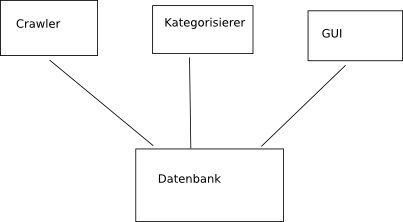
\includegraphics{img/systemmodell.png}
	\caption{Das Systemmodell}
	\label{c:systemmodell}
\end{figure}

\begin{description}
	\item[Crawler] Aufgabe des Crawlers ist es Mithilfer der Twitter-Stream- und Search-API die Twitterdaten zu sammeln. Es sollen verifizierte Benutzer und Retweets von Tweets dieser Nutzer gefunden werden. Diese Daten sollen noch im Crawler lokalisiert werden, bevor sie in der Datenbank abgespeichert werden.
	\item[Kategorisierer] Der Kategorisierer sucht in der Datenbank nach Accounts, denen noch keine Kategorie zugeordnet wurde. Anhand der Daten aus der DMOZ-Datenbank sollen diese Accounts dann hierachisch kategorisiert werden.
	\item[GUI] Die GUI greift lesend auf die Datenbank zu und visualisiert die Daten anhand vom nutzer gegebener Eingaben. Gleichzeitig ist es möglich über die GUI weitere Twitteraccounts (auch nicht verifizierte) in die Datenbank aufzunehmen, so dass auch diese analysiert werden können.
\end{description}


